%!TEX root =  main.tex
%!TEX encoding = UTF-8 Unicode
\chapter{嗜好の予測}
\label{sec:cfcbf}

嗜好の予測とは,活動利用者の嗜好データや,アイテムの特徴を用いて,活動利用者の各アイテムへの関心や好みの度合いを予測することである.

嗜好の予測段階の実現方法は大きく二つに分類される.
レンタルビデオ店で,顧客が見たい映画を推薦する場合を考えてみよう.
一つは,ファンである監督,好みのジャンルを利用者に尋ねてその条件に合ったものを選ぶ方法である.
これを,検索対象の内容を考慮して推薦をするので\term{内容ベースフィルタリング}{content-based filtering}と呼ぶ.
もう一つは,映画の趣味が似ている知り合いに,面白かった映画を教えてもらう「口コミ」の過程を自動化する方法である.
他の人との協調的な作業によって推薦対象を決めるため,この推薦手法は\term{協調フィルタリング}{collaborative filtering}や社会的フィルタリング (social filtering)と呼ばれている.
\index{社会的フィルタリング|see{協調フィルタリング}}\index{social filtering|see{collaborative filtering}}

\begin{figure}
%(a) GroupLens   5.6  10.8  26.1  34.9  22.6
%(b) Amazon.com  7     5     8    20    60
%(c) 寿司        7.9   9.1  22.6  22.7  37.5
\centering
\begin{minipage}{0.6\fullwidth}
\centering
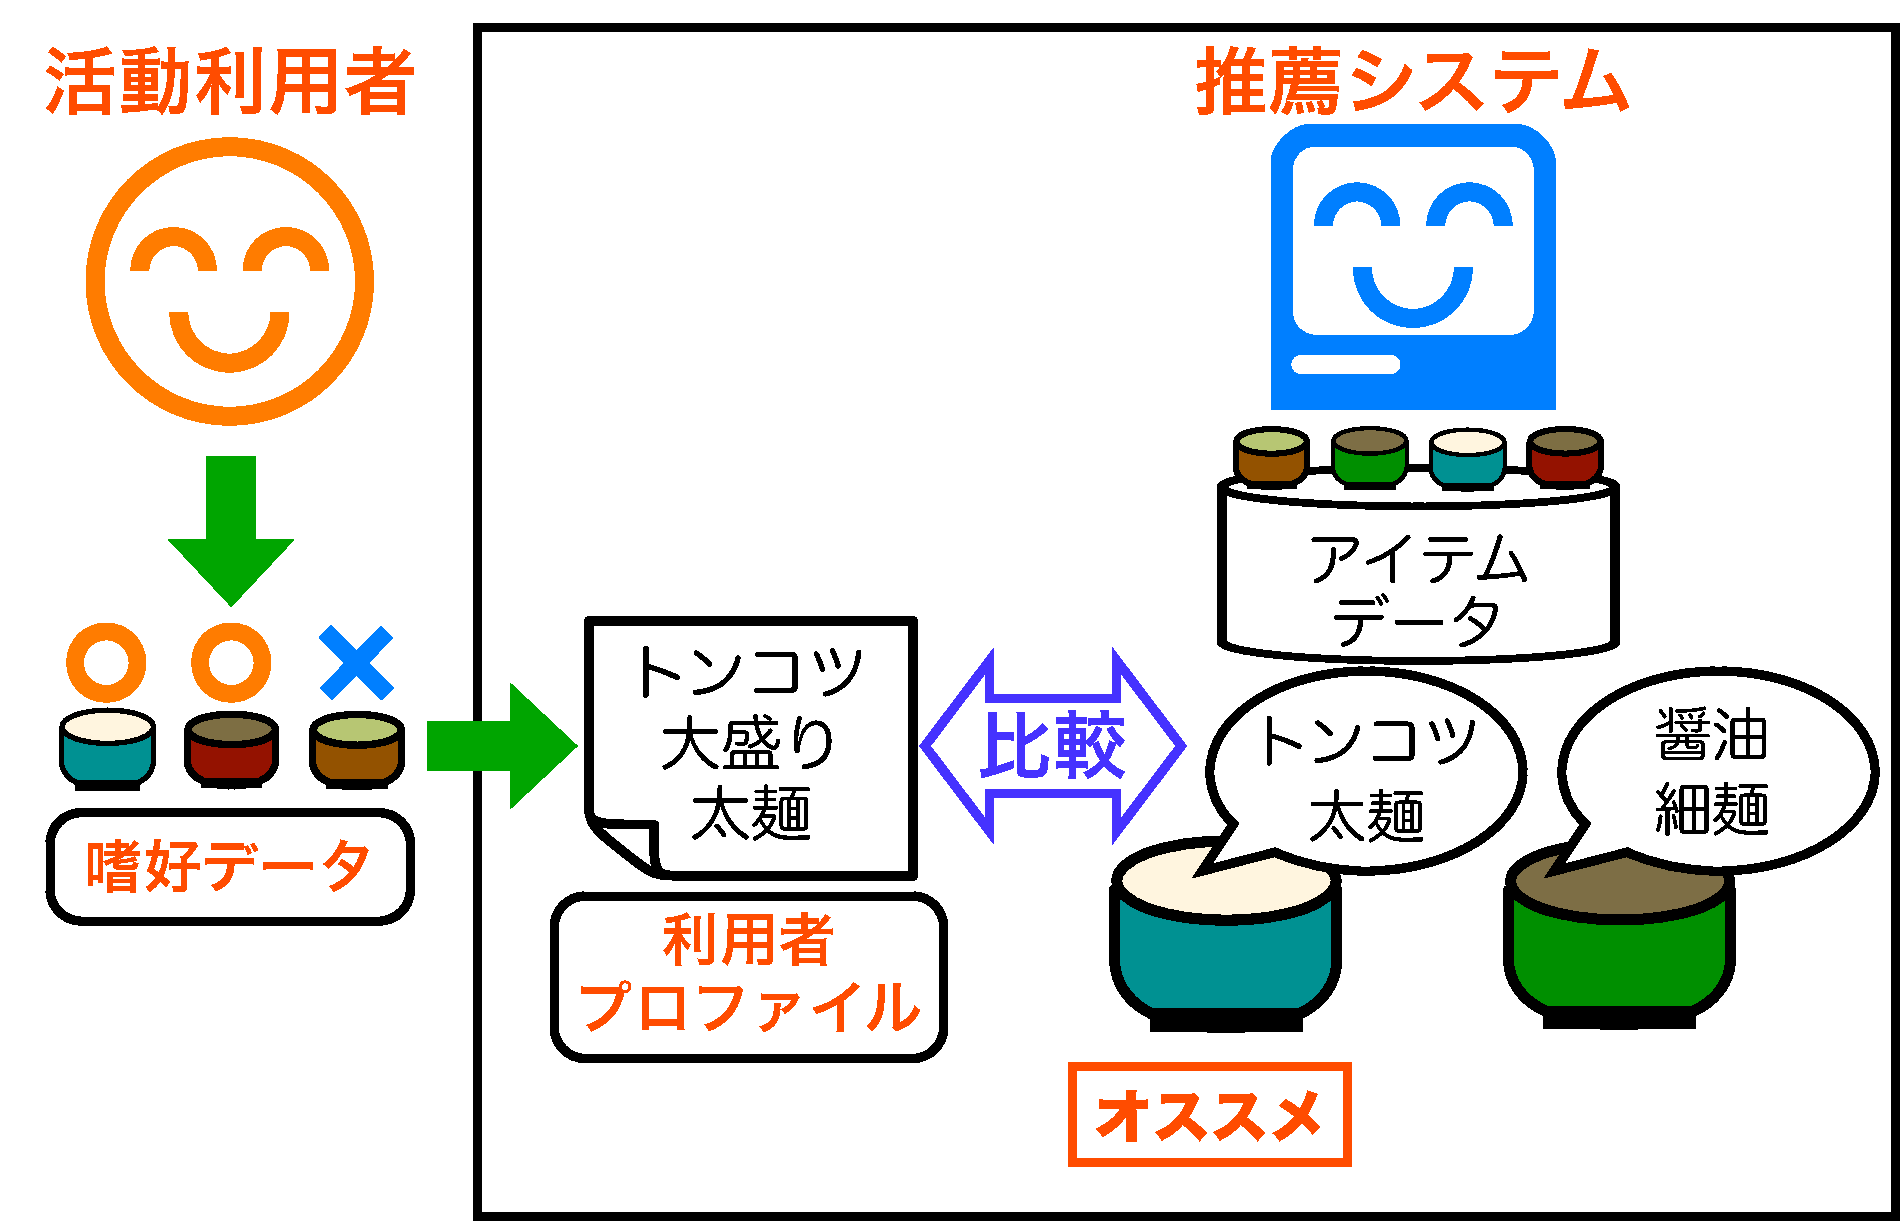
\includegraphics[width=\textwidth]{rsyscategory-icbf.pdf}\\
 (a) 内容ベースフィルタリング(間接指定型)
\end{minipage}\\\medskip
\begin{minipage}{0.6\fullwidth}
\centering
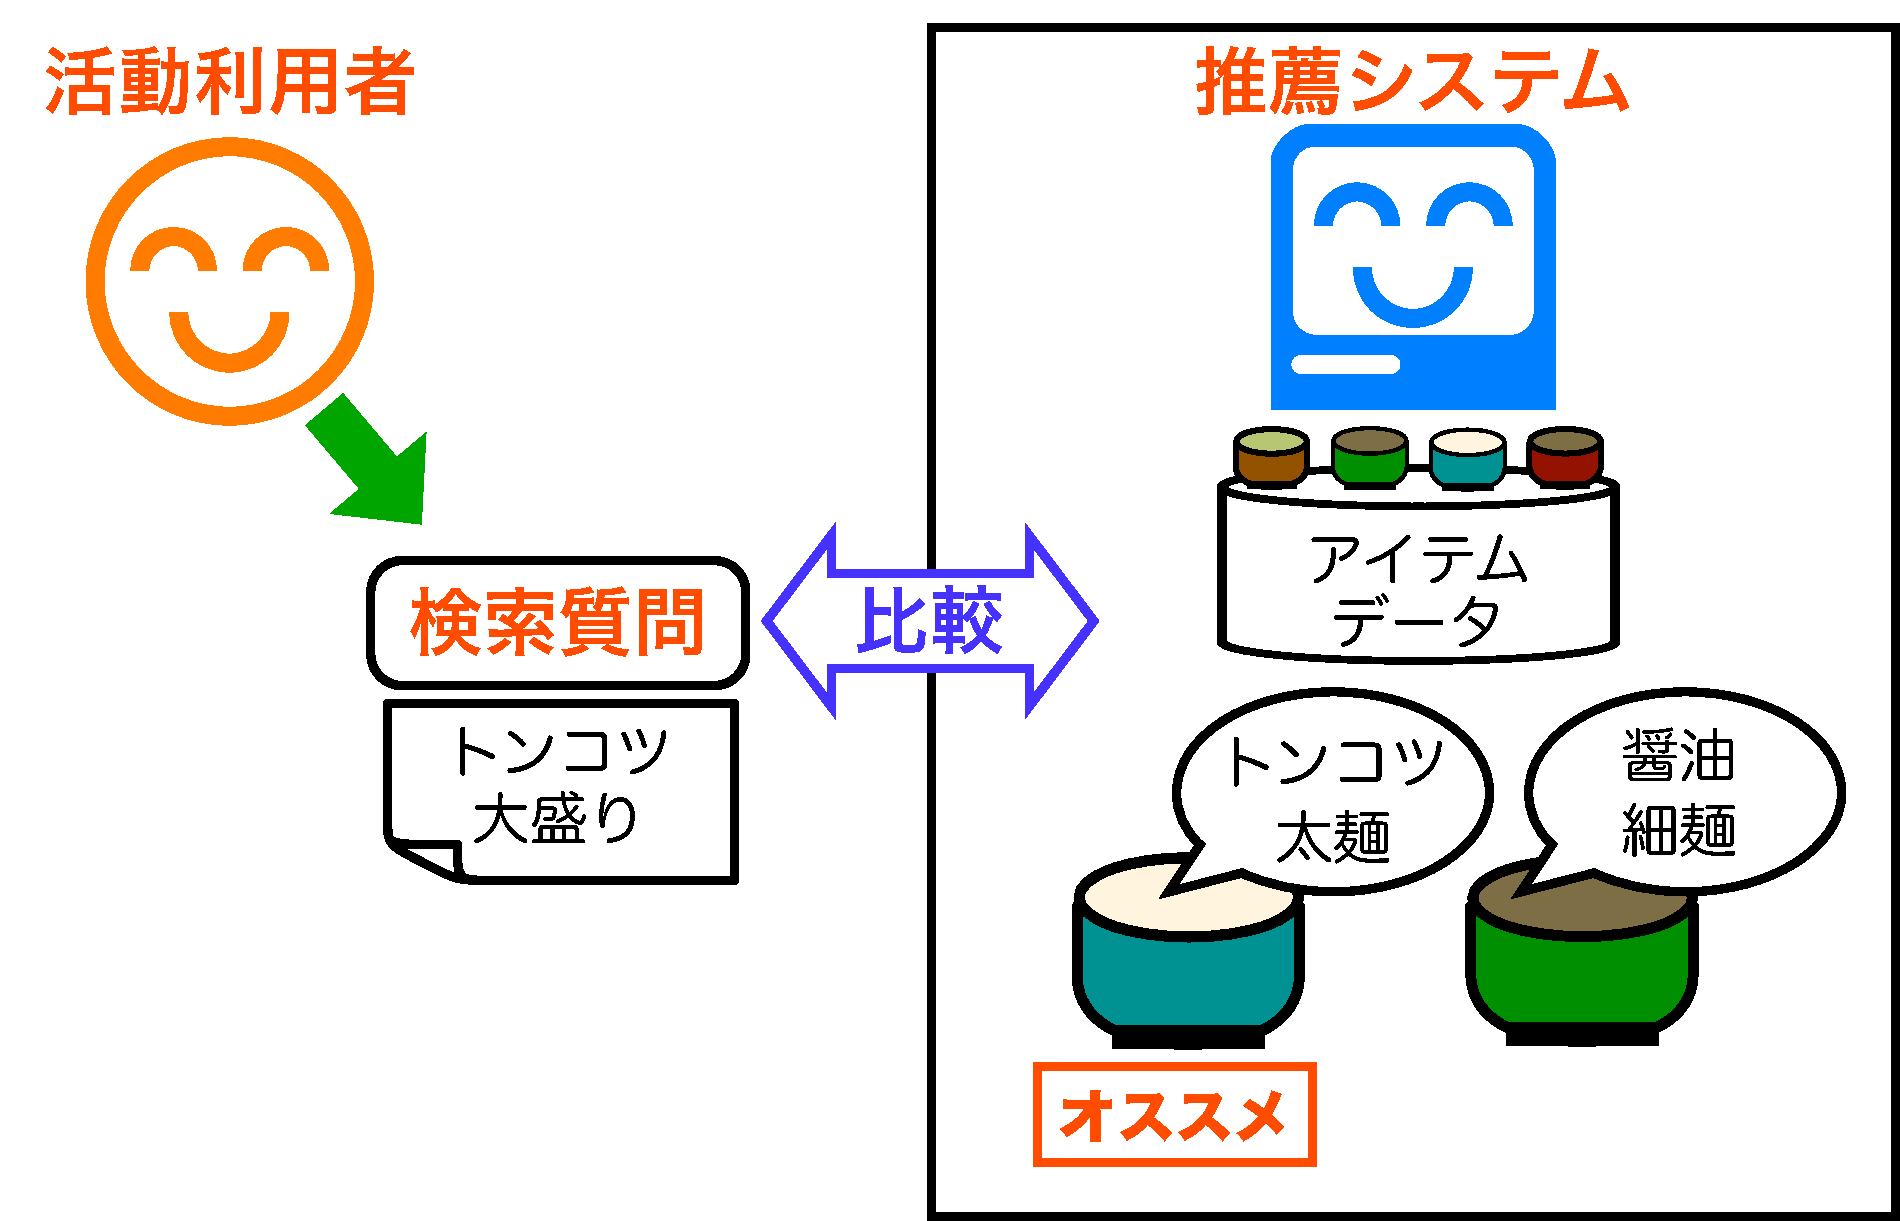
\includegraphics[width=\textwidth]{rsyscategory-dcbf.pdf}\\
 (b)~内容ベースフィルタリング(直接指定型)
\end{minipage}\\\medskip
\begin{minipage}{0.6\fullwidth}
\centering
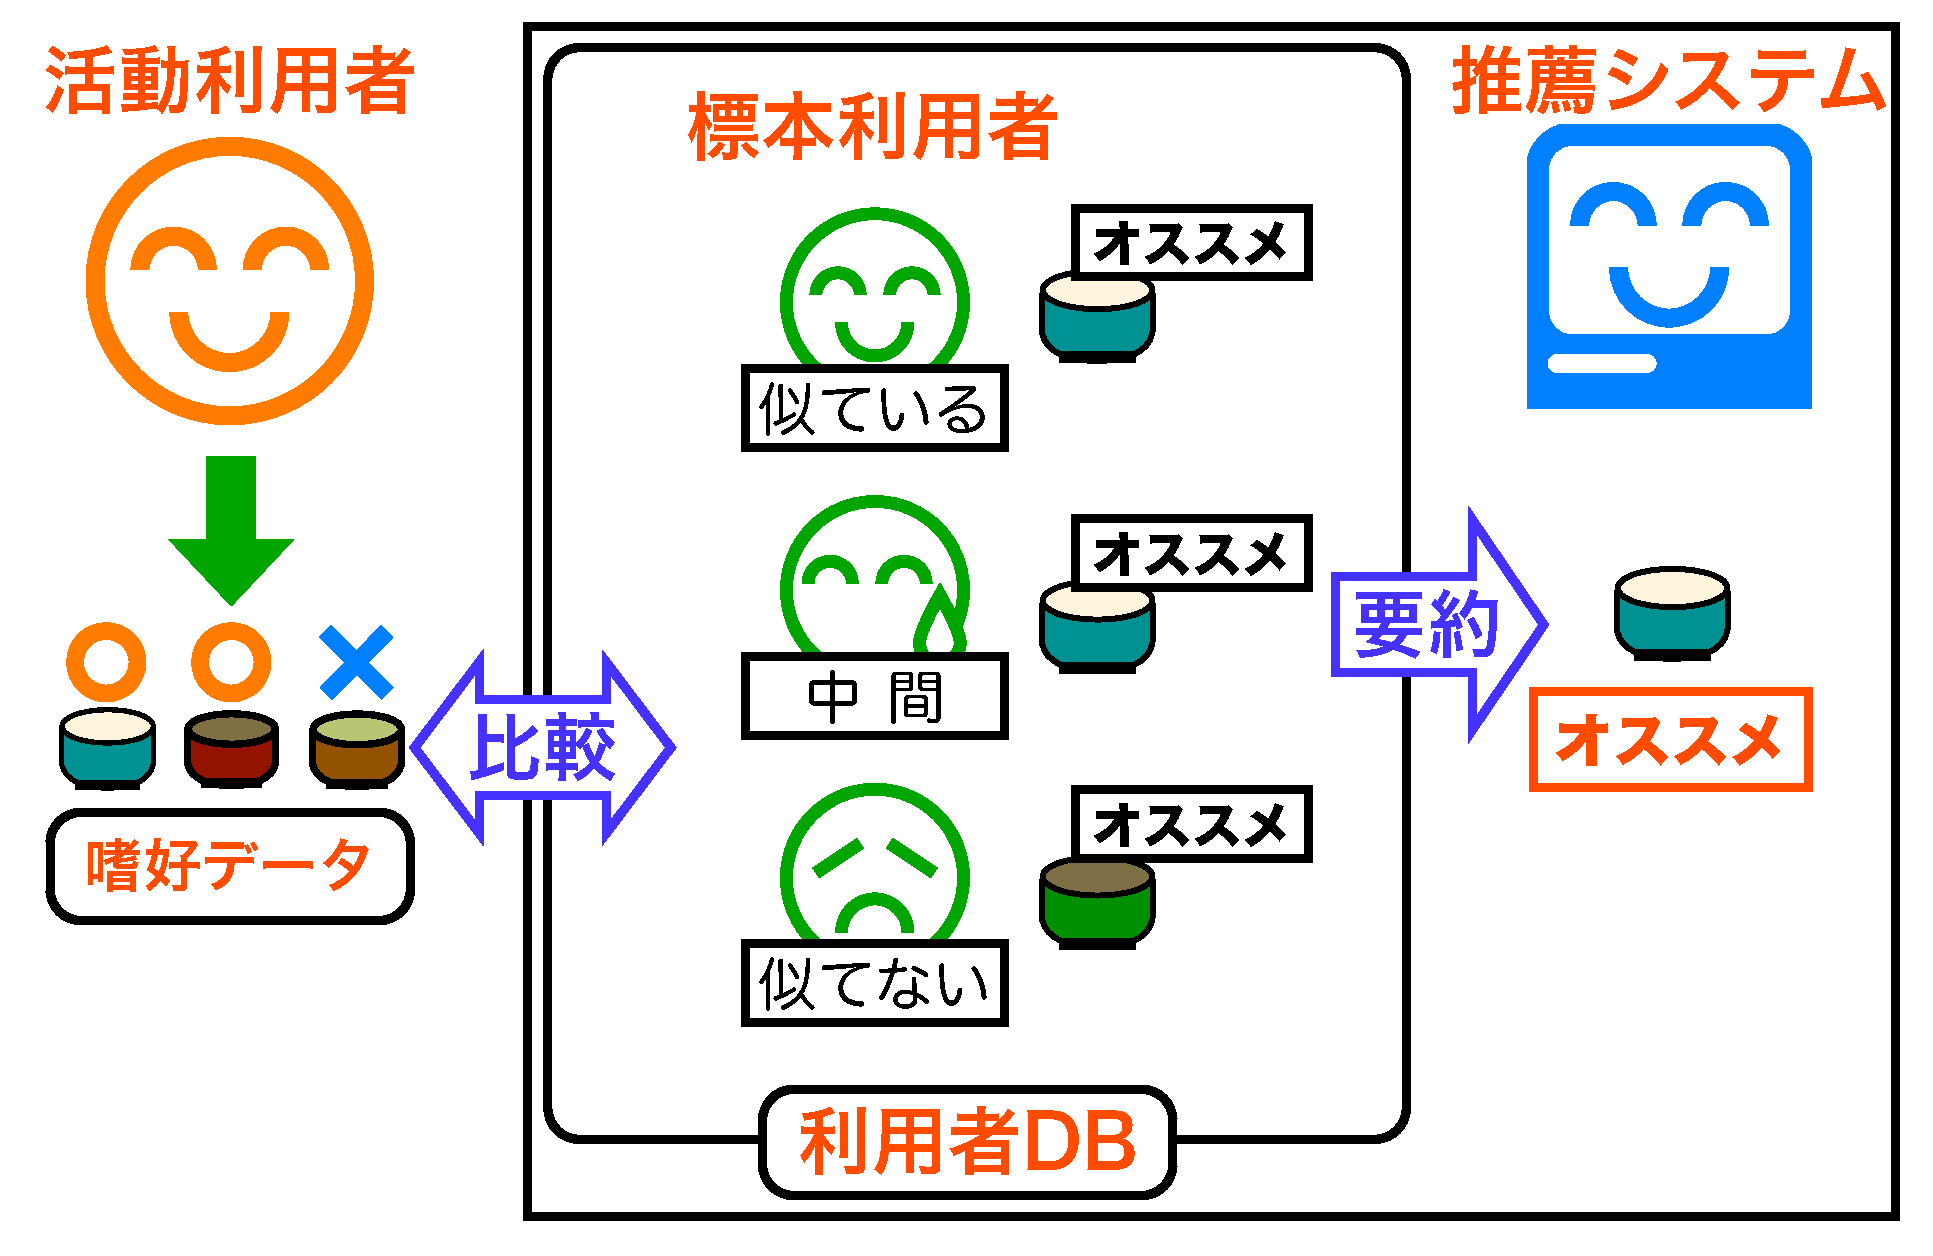
\includegraphics[width=\textwidth]{rsyscategory-cf.pdf}\\
 (c)~協調フィルタリング
\end{minipage}
\caption{内容ベースフィルタリングと協調フィルタリング}
\label{fig:cfcbf}
\end{figure}

現在では,どちらの方法にもいろいろな派生型が提案されているが,純粋な形では\ref{fig:cfcbf}のように予測する.
内容ベースフィルタリング(\ref{fig:cfcbf}(a)と(b))では,アイテムの性質と利用者の嗜好パターンを比較して,利用者が好むと判断したものを推薦する.
このアイテムの性質は特徴ベクトルによって記述される.
特徴ベクトルとは,アイテムのいろいろ側面の性質を表す特徴を集めて,ベクトルの形にしたものである.
各特徴は,事前に定めた定義域中の値をとることで,そのアイテムの性質を表現する.
ラーメンの例を示そう.このとき,スープの種類,麺の太さ,価格といった特徴からなるベクトルでラーメンを表現する.
スープの種類という特徴は,トンコツ,醤油,塩のような定義域の値の一つをとり,価格という特徴では自然数がその定義域となる.
そして,ある特定のラーメン『トンちゃん』があるとすると
\begin{center}
\footnotesize
(スープの種類=トンコツ, 麺の太さ=細麺 ,…, 価格=650円)
\end{center}
といったベクトルで表現される.
こうした情報をいろいろなアイテムについて収集したものをアイテムデータと呼んでおく.
一方,利用者の嗜好パターンは\term{利用者プロファイル}{user profile}によって表す.
この利用者プロファイルを間接指定するシステムと,直接指定するものがある.
間接指定型(\ref{fig:cfcbf}(a))では,利用者のいろいろなアイテムに対する嗜好データ,すなわち,好き嫌いの度合いを定量化したデータを集める.
この嗜好データと,アイテムデータに基づいて,その利用者が好むアイテムの特徴のパターンを機械学習の手法でモデル化し,利用者プロファイルとする.
直接指定型(\ref{fig:cfcbf}(b))では,利用者が明示的に,自身が好むアイテムの特徴を表した検索質問(query)(批評(critique)ともいう)を入力する.
一般的な検索質問は「スープの種類は醤油で,価格は500円以下」といった,特徴に対する制約の形式だが,自然言語文などを扱えるものもある.
この検索質問はそのまま利用者プロファイルとして用いられる.
内容ベースフィルタリングでは,アイテムデータ中のアイテムの特徴ベクトルと,利用者プロファイルとを比較し,プロファイルに最も近い特徴ベクトルをもつアイテムを利用者が好むものと判断して推薦をする.

もう一つの協調フィルタリング(\ref{fig:cfcbf}(c))では,アイテムの性質は全く考慮しない.
その代わりに,システムが利用される前に,多くの利用者の,いろいろなアイテム対する嗜好データをデータベースに集積している.
このデータベースを\term{利用者データベース}{user database}(「利用者DB」と略す)と呼び,この利用者DBに嗜好データを登録している利用者を\term{標本利用者}{sample user}と呼ぶ.
\index{利用者DB|see{利用者データベース}}\index{user DB|see{user database}}
さらに,今までの嗜好パターン,すなわち,どのアイテムを好み,どのアイテムを嫌うのかという傾向が類似している利用者は,これからも同じアイテムを好み,同じアイテムを嫌うであろうという仮定を導入する.
この仮定の下,活動利用者と,嗜好パターンが類似している標本利用者を見つけ,これらの標本利用者が好むものを活動利用者に推薦する.

なお,内容ベースフィルタリングは,いろいろな拡張が行われているので,厳密に定義するのは難しい.
文献\cite{ej:048}では,デモグラフィックな特徴(\ref{sec:featuredata})などを用いず,アイテムの特徴のみを用いた,間接指定型の手法のみを内容ベースフィルタリングと定義している.
そして,上記の直接指定型にあたる知識ベース型や,デモグラフィックな特徴を使うものも,別の種類として細かく分類している.
しかし,細分化しても多種多様な手法を厳密に分類するのは実際には難しいので,本稿では,広義にとらえて,アイテムやデモグラフィックな特徴を利用するような方法は全て内容ベースフィルタリングとして扱う.
一方,これらの特徴を用いず,標本利用者の嗜好データのみを用いる方法を協調フィルタリングとしておく.

第\ref{chap:algorithm}章では,協調フィルタリングと内容ベースフィルタリングの各種手法を順に紹介する.
さらにその後に,これら二つの手法を組み合わせるハイブリッド法について述べたのち,アルゴリズムの選択の指針について述べる.
これらの話題に移る前に,協調フィルタリングと内容ベースフィルタリングの長所と短所をまとめておく.

\section{内容ベースと協調フィルタリングの比較}
\label{sec:cfcbfcomp}

\begin{table}
\centering
\caption{協調フィルタリングと内容ベースフィルタリングの比較}
\label{tab:cfcbfcomp}
\begin{tabular}{l@{\qquad}>{\centering}p{6zw}>{\centering}p{6zw}p{0pt}}\toprule
%\begin{tabular}{l@{\qquad}cc}\toprule
 & 協調 & 内容ベース & \\\midrule
多様性 & ○ & × & \\
ドメイン知識 & ○ & × & \\
%疎なデータ & △ & × & \\
スタートアップ問題 & × & △ & \\
利用者数 & × & ○ & \\
被覆率 & × & ○ & \\
類似アイテム & × & ○ & \\
少数派の利用者 & × & ○ & \\
\bottomrule
\end{tabular}
\end{table}

協調フィルタリングと内容ベースフィルタリングの長所と短所を\cite{macm:97:02,ej:048}などに基づき\ref{tab:cfcbfcomp}にまとめた.
以下,表中の各項目について詳しく述べる.

\subsection{多様性}
\index{diversity}\index{多様性}

\ref{sec:recomtype}で述べた多様性・セレンディピティについては,協調フィルタリングが有利と言われている.
内容ベースフィルタリングでは,利用者自身が知っているアイテムの特徴に,推薦対象が制限されてしまうことが多い.
例えば,映画の場合であれば,過去に見たのと同じジャンルや監督の作品が推薦される.
さらに,類似した内容のアイテムを推薦し,それを利用者が受け入れることで,利用者プロファイルの偏りが一層強化される現象も生じる.
それに対して,協調フィルタリングでは,自身が知らないジャンルや監督でも,他の標本利用者の知識を通じて知ることができる場合がある.
そうしたときには意外性のある,すなわち,セレンディピティがある推薦ができるとされている.

\subsection{ドメイン知識}

協調フィルタリングの最も重要な長所は,アイテムの特徴,すなわち,アイテムの\term{ドメイン知識}{domain knowledge}を全く必要としないことである.
アイテムの特徴ベクトルの設計に伴う困難には次のようなことがある.
\begin{itemize}
 \item
アイテムの特徴についてのデータを集める手間やコストが必要になる.
仕様についてのデータベースが整備されている商品分野は書籍,CDなどに限られている.
たとえ整備されていても,食品の成分表などのように推薦という目的にはあまり役立たないものもある.
それ以外の分野ではデータベースの構築・更新コストが必要になる.
 \item
 アイテムのある性質を表す特徴がないために,適切な推薦ができないことがある.
 例えば,映画の推薦で,自分がファンであるカメラマンの撮る映画を見る利用者がいたとしても,映画の特徴ベクトルに『カメラマン』の特徴がなければ,内容ベースでは適切な推薦ができない.
%テキストを対象とするときは語の頻度がよく利用されるが個々の特徴の質
%は低い.その他,映画などでは,特徴を数十〜数百種類利用するこ
%とは一般に困難で,量的に制限される.このように,特徴の設計に
%は困難が伴う.
 \item
 どの特徴を採用するかということが,利用者の判断に影響を与える.
推薦アイテムの決定に利用された特徴は,利用者の意志決定でより重要視され,そうでない特徴は無視されるようになる副作用を生じることがある\cite{ec:029}.
 \item
 違う分野のアイテムを推薦することが困難である.
 例えば,ある映画が好きでも,内容ベース法では,そのサントラのCDを推薦することは難しい.
 なぜなら,映画とCDは,異なる特徴ベクトルで表現されているためである.
\end{itemize}

%\subsubsection{疎なデータ}
%
%\ref{sec:rsyslimit}で述べたように,推薦システムが扱うデータは疎であ
%る.
%すなわち,推薦対象の数に対する,利用者一人あたりのアイテムに対する
%評価値の数は非常に少ない.
%内容ベースと協調のどちらにとっても疎なデータからの嗜好の予測は困難
%な問題である.
%だが,協調フィルタリングでは,活動利用者の嗜好データの他に,標本利
%用者の嗜好データも利用できる.
%一方,内容ベースでは,活動利用者の嗜好データのみに依存する.
%そのため,データが疎である問題は相対的に内容ベースの方でより一層深刻である.
%さらに
%内容ベースの方法では,推薦時に利用者の嗜好データを新たに要求するな
%どの対処方法がある.

\subsection{スタートアップ問題}
\index{コールドスタート問題|see{スタートアップ問題}}\index{cold-start problem|see{start-up problem}}
\index{ランプアップ問題|see{スタートアップ問題}}\index{ramp-up problem|see{start-up problem}}

\term{スタートアップ問題}{start-up problem}(コールドスタート問題やランプアップ問題とも呼ぶ)は,2種類に分けられる.
一つは,新たにシステムを利用し始めた利用者(first raterやearly raterともいう)に対して適切な推薦をする難しさであり,もう一つは,推薦対象として新たにシステムに導入されたアイテムを推薦する難しさである.
前者については,協調フィルタリングでは,他の標本利用者との類似性を判定できないため良い推薦をするのは難しい.
間接指定型の内容ベースフィルタリングでも,利用者プロファイルが不完全になるためやはり難しい.
加えて,利用者本人の評価値しか利用できないので,問題がさらに深刻になることがある.
だが,直接指定型の内容ベース法では,自身の利用者プロファイルを直接記述するためこうした問題は生じない.
よって,観光地の案内端末での推薦など,同一利用者の継続的な利用があまりない状況では,直接指定型の内容ベース法を採用すべきである.
一方,継続的な利用がなされるならば,嗜好データの蓄積に伴って予測精度が向上する協調フィルタリングや間接指定型の内容ベースフィルタリングがよいであろう.

一方,後者の新規アイテムに対する問題については,内容ベースフィルタリングが優れている.
内容ベースフィルタリングでは,利用者プロファイルがあれば,新規のアイテムでも,その特徴ベクトルを手がかりに,全く問題なく推薦ができる.
しかし,協調フィルタリングでは,標本利用者の評価を利用するので,まだ誰も評価していない新規のアイテムは,推薦を予測する手がかりがなく,そのアイテムに対する活動利用者の好みを判断できない.
以上のことから,商品が頻繁に入れ替わるような場合は,内容ベースフィルタリングが有利である.

\subsection{利用者数}

内容ベース法の場合は,たとえシステムの利用者が一人であっても推薦は可能である.
一方,協調フィルタリングは,他の利用者の意見を参照するので,利用者数がある程度なければ実行できない.
また,利用者が他にいない状況では,適切な推薦もできないため,新たな利用者の増加も難しい.
そのため,電子商取引サイトでのポイントの配布といったインセンティブや,暗黙的な方法で自動収集するといった手段で,十分な規模の嗜好データ量を維持する必要がある.

\subsection{被覆率}
\index{被覆率}\index{coverage}

\ref{sec:recomtype}で述べた被覆率は,適合アイテム列挙タスク(\ref{sec:recomtask})では特に重視すべき評価規準である.
協調フィルタリングでは,まだ誰も評価していないアイテムは推薦の対象にできないため,被覆率を100\%にはできない.
一方,内容ベースでは,アイテムの特徴を手がかりに,全てのアイテムについて推薦すべきかどうかの判定をすることができる.
よって,特徴に欠損値がなければ,被覆率は100\%となる.

\subsection{類似アイテム}

ドメイン知識の項では,アイテムの特徴を使うことの短所を述べたが,アイテムの特徴を使うことの長所もある.
アイテムの性質を無視する協調フィルタリングでは,同じ商品のサイズや色の違うもの,また,同じ目的の競合商品などは全く異なるものとして扱われる.
例えば,利用者AとBは共に,同じサッカーチームのファンであったとしよう.だが,Aはこのチームのロゴのはいったマグカップを,Bはロゴ入りのタオルを買ったとする.
すると,協調フィルタリングでは,チームロゴという特性を明示的に考慮できないので,そのことを推薦に反映できない.
一方,内容ベースフィルタリングでは,利用者Aが過去にマグカップとタオルを購入していれば,アイテムの特徴から,そのサッカーチームのロゴ入りの他のアイテムを推薦することも可能である.

また,推薦されたアイテムを利用者が拒否した場合,それのサイズや色が違うだけの類似アイテムを推薦されてしまう場合も,協調フィルタ
リングでは生じる.
例えば,ある商品を却下したすぐ後で,その商品の色違いを推薦される場合はよく生じうる.
これを回避するには,どのアイテムとどのアイテムを同じとみなすかが重要になる.
すなわち,JANコードなどの商品IDが異なっていても,協調フィルタリングで扱う場合には,色違いなどの類似アイテムは同じアイテムとして扱うようにする必要がある.
しかし,どのアイテムを同じとみなすかは,アイテムのドメイン依存した難しい問題である.
例えば,服飾などでは色の違いは重視されるだろうが,ティッシュペーパなどは色違いでも同じアイテムとみなして良いだろう.

\subsection{少数派の利用者}

協調フィルタリングでは,非常に少数派の嗜好パターンをもつ利用者は,類似した嗜好パターンをもつ利用者を全く,または,ごく少数しか見つけられないので,適切な推薦を受けられない場合がある.
例えば,ほとんど無名なタレントだが,利用者と出身地が同じであるのでファンである人がいたとしよう.
こうした嗜好を持つ人は非常に希であろう.
さらに,そうした人が同じシステムを利用していることはさらに希である.
すると,協調フィルタリングでは,類似した嗜好の人がいなければ嗜好を予測できないので,こうした観点からの推薦は難しい.一方,内容ベースフィルタリングでは,タレントの出身地情報を用いて適切な推薦をすることも可能である.
